\documentclass[12pt]{report}

% Packages to handle math, references, spacing, etc.
\usepackage{amsmath}  % For math equations
\usepackage{amsfonts} % For more fonts
\usepackage{amssymb}  % For more symbols
\usepackage{hyperref} % For hyperlinks
\usepackage{graphicx} % For handling figures
\usepackage{fancyhdr} % For custom headers
\usepackage{geometry} % For page margins and space control
\usepackage{titlesec} % For custom section titles
\usepackage{media9} % For PDF with embedded interactive content

\usepackage{attachfile2}


% Page setup
\geometry{top=5mm, bottom=5mm, left=8mm, right=8mm}  % 3mm margins on all sides
\pagestyle{fancy}  % Enable fancy headers
\fancyhf{} % Clear header and footer
\fancyhead[L]{Mathematics Cheat Sheet} % Header text on left
\fancyfoot[C]{\thepage} % Page number centered at the bottom

% Adjust section and chapter font size
\titleformat{\chapter}[hang]{\normalfont\huge\bfseries}{\thechapter}{2em}{}
\titleformat{\section}[hang]{\normalfont\LARGE\bfseries}{\thesection}{2em}{}
\titleformat{\subsection}[hang]{\normalfont\Large\bfseries}{\thesubsection}{2em}{}

% No identation
\setlength{\parindent}{0pt}

% Custom space for equations: 4mm above and below equations
\newcommand{\spacedequation}[1]{\vspace{4mm}\begin{equation} #1 \end{equation}\vspace{4mm}}

% Chapter and section handling
% \titleclass{\chapter}{standard} % Ensure chapters are on a new page
\newcommand{\chapterbreak}{\newpage} % Force new page at the start of each chapter

% Custom command for adding vertical space
\newcommand{\emptyline}{\vspace*{0.5cm}}

% Hyperlinking for sections, subsections, equations, etc.
\hypersetup{
    colorlinks=true,  % Enable colored links
    linkcolor=blue,   % Set color of links
    urlcolor=blue,    % Set color of URLs
    pdftitle={Mathematics Cheat Sheet}, % PDF metadata
    pdfauthor={Simon F. Roske} % Author name
}

% Make sure figures do not overlap and fit to page
\setlength{\textfloatsep}{10pt plus 1.0pt minus 2.0pt} % Space for floats (figures, tables)
\setlength{\floatsep}{10pt plus 1.0pt minus 2.0pt}    % Space between floats
\setlength{\intextsep}{10pt plus 1.0pt minus 2.0pt}    % Space above/below in-text floats

% Ensure figures are sized properly
\DeclareGraphicsExtensions{.pdf,.png,.jpg}  % Supported file types for figures
\graphicspath{{./figures/}}  % Default path for figures

\begin{document}

\title{Mathematics Cheat Sheet}
\author{Friend}
\date{\today}
\maketitle

% Input chapters
\chapter{Numbers}\label{Numbers}

\section{Natural Numbers $\mathbb{N}$}\label{Natural Numbers}
The set of natural numbers represents the process of counting. Whether or not 0 is part of $\mathbb{N}$ depends on the definition and may vary. If 0 is not included, the set is defined as:

\spacedequation{\mathbb{N} = \{1, 2, 3, 4, \dots, n, n+1, \dots \}.}

How can we perform arithmetic with natural numbers? Addition and multiplication are unrestricted. We say that $\mathbb{N}$ is closed under addition and multiplication. Other operations, such as subtraction and division, are not universally applicable because negative numbers are not part of the natural numbers. A subset of $\mathbb{N}$ is the set of \textbf{prime numbers}, defined as:

\spacedequation{\mathbb{P} = \{1, 2, 3, 5, 7, 11, 13, 17, 19, 23, 29, \dots \}.}

Prime numbers are only divisible by 1 and themselves!

\section{Integers $\mathbb{Z}$}\label{Integers}
The set of integers is obtained by extending the natural numbers to include negative numbers:

\spacedequation{\mathbb{Z} = \{\dots, -3, -2, -1, 0, 1, 2, 3, \dots \}.}

Now subtraction is also possible without restriction.

\section{Rational and Irrational Numbers $\mathbb{Q}$, $\mathbb{R \backslash \mathbb{Q}}$}\label{Rational and Irrational Numbers}
To perform unrestricted division, we need fractions:
\begin{itemize}
    \item \spacedequation{\mathbb{Q}_+ = \left\{ \frac{a}{b} \mid a, b \in \mathbb{N}, b \neq 0 \right\}}
\end{itemize}
Including negative fractions, we get the set of rational numbers:
\begin{itemize}
    \item \spacedequation{\mathbb{Q} = \left\{ \frac{a}{b} \mid a, b \in \mathbb{Z}, b \neq 0 \right\}}
    \item In $\mathbb{Q}$, all basic arithmetic operations are allowed.
    \item $\mathbb{Q}$ includes all positive and negative fractions, as well as all terminating decimal fractions (e.g., -3.75) and repeating decimal fractions (e.g., 0.6666...).
\end{itemize}
One operation is not fully allowed within the rational numbers: taking square roots, since it can lead to infinite numbers that cannot be expressed as fractions. These numbers are called \textbf{irrational numbers}, e.g., 

\spacedequation{\sqrt{2} = 1.41421356\dots}

\section{Real Numbers $\mathbb{R}$}\label{Real Numbers}
By combining the rational and irrational numbers, we get the real numbers $\mathbb{R}$. However, taking square roots of negative numbers is not defined. For example,

\spacedequation{\sqrt{-4}}

is not defined, and such numbers are not included in $\mathbb{R}$.

\section{Complex Numbers $\mathbb{C}$}\label{Complex Numbers}
A complex number \( z \) is represented as a pair of real numbers:

\spacedequation{x + iy \mid x, y \in \mathbb{R}, \quad i = \sqrt{-1}.}

The important feature of the imaginary unit \( i \) is that it allows us to take the square root of negative numbers. A complex number \( z \in \mathbb{C} \) can also be written as the pair \( (x, y) \), where \( x \) is the real part and \( y \) is the imaginary part. Thus, the set of complex numbers $\mathbb{C}$ can be geometrically represented as pairs of real numbers \( (x, y) \) on the complex plane (also called the Gaussian plane), as shown in the figure below.

\begin{figure}[ht]
    \centering
    \includegraphics[width=0.5\textwidth]{../images/Gaußsche_Zahlenebene.png}
    \caption{Gaussian Plane; $c \in \mathbb{C}$ as a real number pair $(x, y)$}
    \label{fig:zahlplane}
\end{figure}

The addition of two complex numbers is defined as:

\spacedequation{z_1 + z_2 = (x_1 + x_2) + (y_1 + y_2) \cdot i}

and the subtraction as:

\spacedequation{z_1 - z_2 = (x_1 - x_2) + (y_1 - y_2) \cdot i.}

Multiplication is defined as:

\spacedequation{z_1 \cdot z_2 = (x_1 + x_2) \cdot (y_1 - y_2) \cdot i = x_1 y_1 + x_1 y_2 \cdot i + y_1 x_2 \cdot i + x_2 y_2 \cdot i^2,}

which simplifies to:

\spacedequation{z_1 \cdot z_2 = (x_1 y_1 - x_2 y_2) + (x_1 y_2 + y_1 x_2) \cdot i.}

If \( z \) is a complex number, then \( z^* \) is its complex conjugate. In the representation below, the real part of \( z \) is reflected. In particular, we have 

\spacedequation{i^* = -i, \quad z^* = x - y \cdot i.}

Multiplying by the complex conjugate gives the magnitude of \( z \):

\spacedequation{|z| = \sqrt{x^2 + y^2}.}

The division of complex numbers is defined as:

\spacedequation{\frac{z_1}{z_2} = \frac{z_1}{z_2} \cdot \frac{z_2^*}{z_2^*}.}

This operation is a bit cumbersome and can be avoided when possible. If it cannot be avoided, multiply the numerator and denominator separately and simplify using the definition of \( i \).

A different representation is possible using polar coordinates:

\spacedequation{z = a + i \cdot b \quad \left. a, b, r \in \mathbb{R}, \theta \in [0, 2\pi] \right| \Leftrightarrow z = r \cdot (\cos(\theta) + i \cdot \sin(\theta)) \Leftrightarrow r \cdot e^{i\theta}.}

\subsection{Special Numbers}\label{Special Numbers}

\subsubsection{$\pi$ - The Circle Constant}\label{Circle Constant}
3.1415926535\dots is the irrational number $\pi$\footnote{Pi's digits omitted for brevity.}. Pi describes the ratio of the circumference to the diameter of a circle. Many formulas involve $\pi$:

\spacedequation{\text{Circumference} \quad U = \pi \cdot d = 2 \cdot \pi \cdot r,}

\spacedequation{\text{Area} \quad A = \pi \cdot r^2,}

\spacedequation{\text{Volume} \quad V = \frac{4}{3} \cdot \pi \cdot r^3.}

\subsubsection{$e$ - Euler's Number}\label{Euler's Number}
Euler's number is the base of the natural logarithm \(\ln(e) = 1\). Euler's number can be approximated as 

\spacedequation{e = 2.71828,}

but like $\pi$, it does not have an exact solution. Named after the Swiss mathematician and physicist Leonhard Euler (1707-1783), \( e \) is crucial for exponential functions.

\chapter{Fundamentals \& Arithmetic Laws}\label{FundamentalArithmeticLaws}

A binary operation can be defined as a way in which two objects determine a third. The operation is abstractly expressed with '$\circ$'. The \textbf{law of closure states} that the result of an operation on two elements of a set is also an element of that set. That allows to define operations such as \textit{addition} and \textit{multiplication}.
Depending on the \textbf{algebraic structure}, operations differ in outcome (e.g. $1 +1 \neq 2 \in \mathbb{F}_{2} = {0,1}$). 
Although operations may yield different outcomes, axioms are fundamental and true for most structures. \textit{Note:} Having to prove a certain law holds for a specific case is often required during exercises in analysis.

\section{Axioms}\label{Axioms}
Axioms establish that algebraic structures have operations (addition and multiplication), and that these operations behave in specific, predictable ways. The most fundamental laws that apply to \textbf{most} structures are:
See this \href{https://math.libretexts.org/Bookshelves/Analysis/Mathematical_Analysis_(Zakon)/02%3A_Real_Numbers_and_Fields/2.01%3A_Axioms_and_Basic_Definitions}{article} for more information.

\subsection{Commutative Law}\label{Commutative Law}

The order of the operation does not matter, e.g., 
\spacedequation{2 \circ 3 = 3 \circ 2}.

\subsection{Associative Law}\label{Associative Law}

The grouping of three numbers does not affect the result of the operation, e.g., 
\spacedequation{(2 \circ 3) \circ 4 = 2 \circ (3 \circ 4)}.

\subsection{Distributive Law}\label{Distributive Law}

The handling of parentheses depends on the number set and the type of operation. For addition and multiplication in the set of real numbers $\mathbb{R}$, both operations are distributive. Thus, 
\spacedequation{2 \odot (3 \oplus 4) = 2 \odot 3 \oplus 2 \odot 4}.

\subsection{Inequality Laws}\label{Inequality Laws}

Inequalities change depending on the operation:
\begin{itemize} \item Adding/subtracting a constant: \spacedequation{a > b \Rightarrow a + c > b + c} \item Multiplying by a positive constant: \spacedequation{a > b \Rightarrow a \cdot c > b \cdot c} \item Multiplying by a negative constant reverses the inequality: \spacedequation{a > b \Rightarrow a \cdot (-c) < b \cdot (-c)} \end{itemize}

\subsection{Identity Laws}\label{Identity Laws}

These laws describe the neutral element in an operation:
\begin{itemize} \item For addition: \spacedequation{a + 0 = a} \item For multiplication: \spacedequation{a \cdot 1 = a} \end{itemize}

\subsection{Inverse Laws}\label{Inverse Laws}

These laws describe how to reverse an operation:
\begin{itemize} \item For addition: \spacedequation{a + (-a) = 0} \item For multiplication: \spacedequation{a \cdot a^{-1} = 1,} where 
$a{-1} = \frac{1}{a}$ and $a \neq 0$
\end{itemize}

\subsection{Zero Laws}\label{Zero Laws}

The number zero has special properties:
\spacedequation{a \cdot 0 = 0} 
Division by zero is undefined.


\subsection{Absolute Value Properties}\label{Absolute Value Properties}

The absolute value represents the distance from zero:
\begin{itemize} \item \spacedequation{|a| \geq 0} \item \spacedequation{|a| = a} \item \spacedequation{|a \cdot b| = |a| \cdot |b|.} \end{itemize}

\section{The Binomial Formulas}\label{Binomial Formulas}

\begin{enumerate}
    \item[(a)] \spacedequation{(a + b)^2 = a^2 + 2ab + b^2}
    \item[(b)] \spacedequation{(a - b)^2 = a^2 - 2ab + b^2}
    \item[(c)] \spacedequation{(a + b) \cdot (a - b) = a^2 - b^2}
\end{enumerate}

\section{Set Operations}\label{Set Operations}

In set operations, the following laws hold:
\begin{itemize} \item Commutative: \spacedequation{A \cup B = B \cup A} \spacedequation{A \cap B = B \cap A} \item Associative: \spacedequation{(A \cup B) \cup C = A \cup (B \cup C)} \spacedequation{(A \cap B) \cap C = A \cap (B \cap C)} \item Distributive: \spacedequation{A \cap (B \cup C) = (A \cap B) \cup (A \cap C)} \end{itemize}

\section{Powers}\label{Powers}

A power is a shorthand notation for repeated multiplication by itself.

\begin{itemize}
    \item \spacedequation{a^0 = 1}
    \item \spacedequation{a^1 = a}
    \item \spacedequation{a^{-1} = \frac{1}{a}}
    \item \spacedequation{a^{-n} = \frac{1}{a^n}}
    \item \spacedequation{a^n = \frac{1}{a^{-n}}}
    \item \spacedequation{a^p \cdot a^q = a^{p+q}}
    \item \spacedequation{a^p : a^q = a^{p-q}}
    \item \spacedequation{a^q \cdot b^q = (a \cdot b)^q}
    \item \spacedequation{a^q : b^q = (a : b)^q}
    \item \spacedequation{(a^p)^q = a^{p \cdot q}}
    \item \spacedequation{\frac{a^m}{a^n} = a^{m-n}}
    \item \spacedequation{\frac{a^n}{b^n} = \left(\frac{a}{b}\right)^n}
    \item \spacedequation{\left(\frac{a}{b}\right)^{-n} = \left(\frac{b}{a}\right)^n}
\end{itemize}

Building on the basic exponent rules, we have: \begin{itemize} \item \spacedequation{(a \cdot b)^n = a^n \cdot b^n} \item \spacedequation{\left(\frac{a}{b}\right)^n = \frac{a^n}{b^n}} \end{itemize}

\section{Roots}\label{Roots}

The root of a number, when multiplied by itself, gives the number. By default, this refers to square roots, but higher roots (e.g., cubic roots $\sqrt[3]{x}$) are also possible. In terms of powers, the square root is expressed as 
\spacedequation{\sqrt{x} = x^{\frac{1}{2}}} 
and 
\spacedequation{\sqrt[n]{x} = x^{\frac{1}{n}}} 
e.g.
\spacedequation{\sqrt[3]{125} = 125^{\frac{1}{3}}.}
If a power has a solution, then 
\spacedequation{x^n = a \Leftrightarrow x = \sqrt[n]{a}}
as in 
\spacedequation{3^4 = 81 \equiv \sqrt[4]{81} = 3.}

Roots also follow these additional rules: \begin{itemize} \item Nested roots: \spacedequation{\sqrt[m]{\sqrt[n]{a}} = \sqrt[m \cdot n]{a}} \item For products: \spacedequation{\sqrt[m]{a \cdot b} = \sqrt[m]{a} \cdot \sqrt[m]{b}} \end{itemize}

\textit{Note:} The nth root is the inverse function of the power function $x^n$.

\section{Logarithms}\label{Logarithms}

\textbf{Question:} What number must I raise \( a \) to, to get \( y \)? Written as 
\spacedequation{\log_a(x) = y.}
\textit{Note:} The logarithms of zero and negative numbers are not defined!

The logarithm is the inverse function of the exponential function:

\spacedequation{f(x) = a^x = y, \quad f^{-1}(y) = \log_a(y) = x.}

Thus, the logarithm provides the exponent of the exponential function to the base \( a \). For the exponential function \( f(x) = e^x \) with \( e \) as the base, the natural logarithm (\(\ln\)) is defined as 
\spacedequation{f^{-1}}.

Logarithms have specific rules:
\begin{itemize}
    \item \spacedequation{\log_a(1) = 0}
    \item \spacedequation{\log_a(a) = 1}
    \item \spacedequation{\log_a(p \cdot q) = \log_a(p) + \log_a(q)}
    \item \spacedequation{\log_a\left(\frac{p}{q}\right) = \log_a(p) - \log_a(q)}
    \item \spacedequation{\log_a(p^q) = q \cdot \log_a(p)}
    \item \spacedequation{\log_a\left(\sqrt[n]{p}\right) = \frac{\log_a(p)}{n}}
    \item \spacedequation{\log_a(p) = \frac{\log_b(p)}{\log_b(a)}}
\end{itemize}

These additional rules expand on logarithmic behavior: \begin{itemize} \item Change of base: \spacedequation{\log_b(a) = \frac{\ln(a)}{\ln(b)}} \item Reciprocal property: \spacedequation{\log_a\left(\frac{1}{b}\right) = -\log_a(b)} \end{itemize}

Logarithmic scaling is helpful when data varies significantly or when relative differences between values are important. Logarithmic scaling makes patterns easier to discern.
 
\chapter{Probability}\label{Probability}


\section{Introduction}\label{Introduction}

\subsection{Basic Concepts and Terminology}

\subsubsection{Sample Space (S)}
The set of all possible outcomes of a random experiment.

\subsubsection{Event (E)}
A subset of the sample space, representing a specific outcome or a group of outcomes.

\subsubsection{Types of Events}
\paragraph{Simple Events}
Events consisting of a single outcome.

\paragraph{Compound Events}
Events consisting of two or more outcomes.

\paragraph{Mutually Exclusive Events}
Two events \( A \) and \( B \) are mutually exclusive if they cannot occur simultaneously, i.e., \( A \cap B = \emptyset \).

\paragraph{Independent Events}
Events \( A \) and \( B \) are independent if the occurrence of one does not affect the probability of the other, i.e.,
\spacedequation{P(A \cap B) = P(A) \cdot P(B).}

\paragraph{Complementary Events}
The complement of event \( A \), denoted by \( A^c \), includes all outcomes in \( S \) that are not in \( A \). The relationship is given by:
\spacedequation{P(A^c) = 1 - P(A).}

\subsubsection{Fundamental Principle of Counting} If an event can occur in \( m \) ways and another event can occur in \( n \) ways, the total number of ways both events can occur is \( m \cdot n \).
    
\subsubsection{Permutations} The number of ways to arrange \( r \) objects from a set of \( n \) distinct objects:
\spacedequation{nPr = \frac{n!}{(n-r)!}.}

\subsubsection{Combinations} The number of ways to choose \( r \) objects from a set of \( n \) distinct objects, without regard to order:
\spacedequation{nCr = \frac{n!}{r!(n-r)!}.}


\subsection{Random Variable}\label{Random Variable}
A random variable is a variable that takes on different numerical values based on the outcome of the event. It is a function that assigns a real number to each possible outcome in the sample space. Random variables can be classified into two types: discrete and continuous.

A \textbf{Discrete Random Variable} takes on a countable number of distinct values. Examples include the number of heads in a series of coin tosses or the number of students present in a class.

A \textbf{Continuous Random Variable} takes on an infinite number of possible values within a given range. Examples include the height of students in a class or the time it takes to run a marathon.

Mathematically, a random variable $X$ can be defined as a function $X: \Omega \rightarrow \mathbb{R}$, where $\Omega$ is the sample space of the random experiment, and $\mathbb{R}$ is the set of real numbers.

\subsection{Dependent and independent variables}\label{Dependent and independent variables}
The probability distribution of a random variable describes how probabilities are assigned to its possible values. For discrete random variables, this is given by the probability mass function (PMF), and for continuous random variables, it is given by the probability density function (PDF).

The independent variable is the factor that a researcher manipulates, while the dependent variable is the outcome that is measured to see the effect of the independent variable.

In an experiment, the independent variable is the variable that is changed or controlled to test the effects on the dependent variable. The dependent variable is the variable being tested and measured. For example, in a study to determine the effect of different amounts of sunlight on plant growth, the amount of sunlight is the independent variable, and the growth of the plant is the dependent variable.

Mathematically, if $X$ is the independent variable and $Y$ is the dependent variable, the relationship can be expressed as:
\spacedequation{Y = f(X),}
where $f$ is a function that describes how $Y$ depends on $X$.

\textit{Note:} There might a multiple dependent variables ($n$) that determine $Y$. Furthermore, there are also multiple observations ($i$) in most cases, such that the extended notation should become familiar:

\spacedequation{Y^i = f(X_n^i), \quad \forall n = 1, \ldots, n.}

Regression analysis can be used to model the relationship between the independent and dependent variables. In simple linear regression, the relationship is modeled as:
\spacedequation{Y = \beta_0 + \beta_1 X + \epsilon,}
where $\beta_0$ is the intercept, $\beta_1$ is the slope, and $\epsilon$ is the error term.

More on exact methods to determine the meaning of such relations is discussed later in \textit{statistics}.

\subsection{Kolmogorov's Axioms}\label{Kolmogorov's Axioms}
Kolmogorov's three axioms are the most well-known description of the fundamental properties of probability theory. Let $\Omega = \{\omega_1, \omega_2, \omega_3, \omega_4, \omega_5, \omega_6\}$ be the sample space of a random experiment, $A$ and $B$ subsets of $\Omega$, and $P$ a function that assigns a real number between 0 and 1 to each $A$. $P(A)$ is called probability if the following three conditions (axioms) are met:
\begin{enumerate}
    \item $P(A) \geq 0$: This condition states that the probability of any subset of $\Omega$ (event) is non-negative. This property is also called non-negativity.
    \item $P(\Omega) = 1$: The second axiom further restricts the range of values of the function $P$. With axioms 1 and 2, $P(A)$ can take any value between 0 and 1.
    \item $P(A \cup B) = P(A) + P(B)$ for disjoint sets $A$ and $B$: This means that no outcome satisfies both events. $A$ and $B$ are called disjoint in this case.
\end{enumerate}

\subsection{Joint, marginal and conditional}\label{Joint, marginal and conditional}

\subsubsection{Probability Formulas}\label{Probability Formulas}

In probability theory, there are various concepts that help us understand the relationships between different events or variables. These include joint probability, marginal probability, and conditional probability. The joint probability $P(X, Y)$ gives the probability that both event X and event Y occur. It can be calculated by the \textbf{product rule}:

\spacedequation{P(X, Y) = P(X|Y) \cdot P(Y) = P(Y|X) \cdot P(X).}

The marginal probability (or 'total probability') $P(X)$ is the probability that event X occurs, regardless of other events. It can be calculated by summing the joint probabilities over all possible values of Y (i.e. \textbf{the sum rule}):

\spacedequation{P(X) = \sum_{y} P(X, Y=y) = \sum_{y} P(X|Y=y) \cdot P(Y=y).}

The conditional probability $P(X|Y)$ gives the probability that event X occurs given that event Y has occurred. It can be calculated by dividing the joint probability of X and Y by the probability of Y:

\spacedequation{P(X|Y) = \frac{P(X, Y)}{P(Y)}.}

If a third variable Z is present, these formulas can be extended to calculate conditional and joint probabilities considering Z. For example, the joint probability of X and Y given Z is defined as:

\spacedequation{P(X, Y|Z) = P(X|Y, Z) \cdot P(Y|Z) = P(Y|X, Z) \cdot P(X|Z).}

And the conditional probability of X given Y and Z is defined as:

\spacedequation{P(X|Y, Z) = \frac{P(X, Y|Z)}{P(Y|Z)}}

with $Y$ and $Z$ being variable. For an arbitrary number of variables \(X_1, X_2, \ldots, X_n\), the joint probability given \(Z\) can be extended as:

\spacedequation{P(X_1, X_2, \ldots, X_n | Z) = P(X_1 | X_2, \ldots, X_n, Z) \cdot P(X_2 | X_3, \ldots, X_n, Z) \cdots P(X_{n-1} | X_n, Z) \cdot P(X_n | Z).}

Similarly, the conditional probability of \(X_1\) given \(X_2, \ldots, X_n\) and \(Z\) is:

\spacedequation{P(X_1 | X_2, \ldots, X_n, Z) = \frac{P(X_1, X_2, \ldots, X_n | Z)}{P(X_2, \ldots, X_n | Z)}.}

\begin{figure}
    \centering
    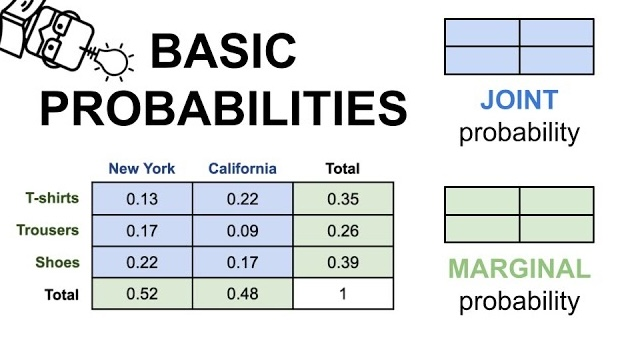
\includegraphics[width=0.5\textwidth]{../images/plot_joint_marginal_conditional.png.jpg}
    \caption{Joint and Marginal, and Conditional Probability. Can you imagine the coloring for the last? \url{https://www.youtube.com/watch?v=xu-HhF3SpbEs}.}
    \label{fig:joint_marginal_conditional}
\end{figure}

\subsubsection{Conditional Independence}\label{Conditional Independence} 
Conditional independence occurs when the occurrence of event X has no effect on the probability of event Y given event Z. In other words, X and Y are conditionally independent if the conditional probability of Y given X and Z is equal to the conditional probability of Y given Z. This is mathematically expressed by the equation 
\spacedequation{P(Y|X,Z) = P(Y|Z).}
If X and Y are independent given Z, it is written as 
\spacedequation{P(X,Y|Z) = P(X|Z) \cdot P(Y|Z).}

\subsubsection{Independence of Variables}\label{Independence of Variables} 
Two variables X and Y are independent if the occurrence of one variable has no effect on the probability of the occurrence of the other variable. Mathematically, this means that the joint probability of X and Y is equal to the product of the individual probabilities of X and Y:
\spacedequation{P(X,Y) = P(X) \cdot P(Y).}
If X and Y are independent, it also holds that \spacedequation{P(X|Y) = P(X).}

\subsection{Bayes}\label{Bayes}
Bayes' theorem makes statements about probabilities given that one knows data or observations, moving from events ($Data$) to their causes (parameters $\Theta$). The more data there is, the more reliable the probability distribution of a variable becomes. Bayes' theorem states:

\spacedequation{P(\Theta|Data) = \frac{P(Data|\Theta) \cdot P(\Theta)}{P(Data)}.}

Here, $P(\Theta|Data)$ is the \textbf{posterior} probability of the parameters given the data. $P(Data|\Theta)$ is the \textbf{likelihood} of observing the data given the parameters. For $P(\Theta)$, one usually sets a \textbf{prior}, that is, its probabilities without prior knowledge.

\emptyline
\textit{Note: It is a good exercise to derive Bayes' theorem from the definition of conditional probability \url{http://www.hep.upenn.edu/~johnda/Papers/Bayes.pdf}.}
\emptyline

Let us consider the so-called "Monty Hall Problem". In this game, there are three doors, behind one of which is a prize, and behind the other two are goats. The player selects a door, and the host opens another door behind which there is a goat. The player then has the option to stay with their original choice or to switch. The question is: Should the player stay with their original choice? Using Bayes' theorem, this question can be clearly answered.
Let $A$ be the chosen door and $C$ the door that the host opens. What is the probability that the prize is behind door $A$, given that $C$ was opened, and what is it for door $B$? We need to calculate $P(A|C)$ and $P(B|C)$. If $P(B|C) > P(A|C)$, one should switch! We know that $P(A) = P(B) = P(C) = \dfrac{1}{3}$, and that only one door is opened behind which there is not the prize. It holds:

\spacedequation{P(A|C) = \frac{P(C|A) \cdot P(A)}{P(C)} = \frac{P(C|A) \cdot P(A)}{P(C|A) \cdot P(A) + P(C|B) \cdot P(B) + P(C|C) \cdot P(C)},}

where $P(C)$ normalizes the probabilities according to the principle of total probability (the sum of all probabilities under which $C$ is opened in our case). Substituting the values, we obtain:

\spacedequation{P(A|C) = \frac{0.5 \cdot \dfrac{1}{3}}{0.5 \cdot \dfrac{1}{3} + 1 \cdot \dfrac{1}{3} + 0 \cdot \dfrac{1}{3}} = \dfrac{1}{3}.}

To understand the logic, ask the question: \textit{How likely is it to open door $X$, given that the prize is behind door $Y$?} On the other hand:

\spacedequation{P(B|C) = \frac{P(C|B) \cdot P(B)}{P(C)} = \frac{P(C|B) \cdot P(B)}{P(C|B) \cdot P(B) + P(C|A) \cdot P(A) + P(C|C) \cdot P(C)}}

\spacedequation{= \frac{1 \cdot \dfrac{1}{3}}{1 \cdot \dfrac{1}{3} + 0.5 \cdot \dfrac{1}{3} + 0 \cdot \dfrac{1}{3}} = \dfrac{2}{3}}

And thus greater for $B$, so one should switch.

Therefore, using Bayes' theorem, we find that the probability of winning by switching doors is $\dfrac{2}{3}$, while the probability of winning by staying is only $\dfrac{1}{3}$. This counterintuitive result demonstrates the power of Bayesian reasoning in updating probabilities based on new information.

Bayes' theorem is widely used in various fields such as statistics, machine learning, medicine, and engineering. It allows for the updating of beliefs in light of new evidence, making it a fundamental tool for probabilistic inference.

In practical applications, Bayes' theorem helps in situations where one needs to determine the probability of a hypothesis given observed data. For example, in medical diagnostics, Bayes' theorem can be used to calculate the probability of a disease given a positive test result, taking into account the prior probability of the disease and the accuracy of the test.

Bayesian methods also play a crucial role in modern data science and machine learning algorithms, such as Bayesian networks and Bayesian inference, which provide a probabilistic approach to reasoning under uncertainty.

\section{Distributions}\label{Distributions}
Probability distributions describe how probabilities are assigned to different outcomes of a random variable. They are categorized into discrete and continuous types.
A \textbf{Discrete Random Variable} has a finite or countable number of possible values, such as the outcomes of a coin toss or a die roll.
A \textbf{Continuous Random Variable} has an infinite number of possible values within a given range, such as hair length measured with increasing precision.
The \textbf{Probability Density Function} (PDF) describes the likelihood of a continuous random variable taking on a particular value. The total area under the PDF curve is 1, representing the total probability. Since the probability of a single value is effectively zero, probabilities are calculated over intervals using integration, resulting in the cumulative distribution function (CDF).

\emptyline
Key concepts include the expected value $E$, variance $V$ (with standard deviation $\sqrt{V}$).
\begin{itemize}
    \item[] \textbf{Expected Value (Mean)}: 
    \begin{itemize}
        \item[] For a discrete random variable \( X \) with possible values \( x_i \) and probabilities \( P(x_i) \):
        \spacedequation{E(X) = \sum_{i=1}^{n} x_i \cdot P(x_i).}
        
        \item[] For a continuous random variable \( X \) with probability density function \( f(x) \):
        \spacedequation{E(X) = \int_{-\infty}^{\infty} x \cdot f(x) \, dx.}
    \end{itemize}
    
    \item[] \textbf{Variance}: 
    \begin{itemize}
        \item[] For a discrete random variable \( X \):
        \spacedequation{\text{Var}(X) = E[(X - \mu)^2] = \sum_{i=1}^{n} (x_i - \mu)^2 \cdot P(x_i).}
        
        \item[] For a continuous random variable \( X \):
        \spacedequation{\text{Var}(X) = E[(X - \mu)^2] = \int_{-\infty}^{\infty} (x - \mu)^2 \cdot f(x) \, dx.}
    \end{itemize}
    
    \item[] \textbf{Standard Deviation}: The standard deviation \( \sigma \) is the square root of the variance:
    \spacedequation{\sigma = \sqrt{\text{Var}(X)}.}
\end{itemize}


\section{Continuous Distributions}\label{Continuous Distributions}

\subsection{Normal Distribution}\label{Normal Distribution}
The normal distribution is also called the Gaussian bell curve. The two parameters ($\mu$ and $\sigma$) represent the mean and standard deviation of the normal distribution. The central limit theorem states that under certain general conditions, the sum of n independent, identically distributed random variables is again normally distributed.

As an example, let's consider rolling n fair dice: If you roll only one die, each face value is equally likely. However, if you roll n dice, the average face value is described by the normal distribution.

Therefore, the normal distribution is the most important, as natural phenomena with sufficiently large n approximate it. The formula for calculating the distribution is:
\spacedequation{f(x,\mu, \sigma) = \frac{1}{\sigma \sqrt{2\pi}} \cdot e^{-\frac{1}{2} \left( \frac{x - \mu}{\sigma} \right)^2}.}

It holds that $E=\mu$ and $V=\sigma^2$ (variance $V$ and standard deviation $\sigma$). The total area enclosed by the curve of the normal distribution is always 1. If $\mu=0$ and $\sigma=1$, it is called the standard normal distribution, which is described by a simplified equation (since $\mu=0$ and $\sigma=1$):
\spacedequation{f(x) = \frac{1}{\sqrt{2\pi}} e^{-\frac{1}{2} x^2}.}

The prefactor ensures that the total area under the curve (and thus the integral from $-\infty$ to $\infty$) is exactly 1. The $\frac{1}{2}$ in the exponent of the exponential function gives the normal distribution a unit variance. Every normal distribution is a variant of the standard normal distribution with scaled standard deviation ($\frac{1}{\sigma}$) and \textit{z-transformed} $\frac{x - \mu}{\sigma}$. The normal distribution is usually written as: $\mathcal{N}(\mu, \sigma^2)$.

\begin{figure}[h]
    \centering
    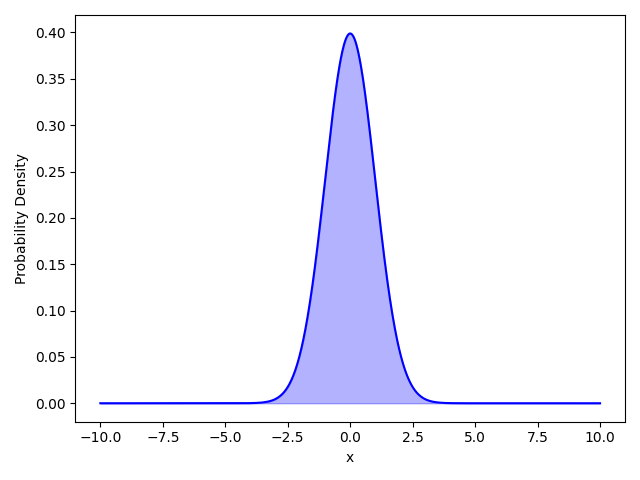
\includegraphics[width=0.5\textwidth]{../images/plot_normal_distribution.png}
    \caption{Normal Distribution with $\mu=0$ and $\sigma=1$}
    \label{fig:normal_distribution}
\end{figure}


\subsubsection{Mixed Distribution}\label{Mixed Distribution}
A mixed distribution consists of several subsets that together form a larger distribution. Such an approach can be used to model a large population with different subpopulations, each of which has individual characteristics. Formally, for each subpopulation $z$, a specific distribution $P(X\mid Z=z)$ is provided. These are mixed according to the probability $P(Z=z)$ of selecting an individual from this subpopulation, i.e.,
\spacedequation{P(X=x) = \sum_{z} P(Z=z)\cdot P(X=x\mid Z=z).}

\begin{figure}[h]
    \centering
    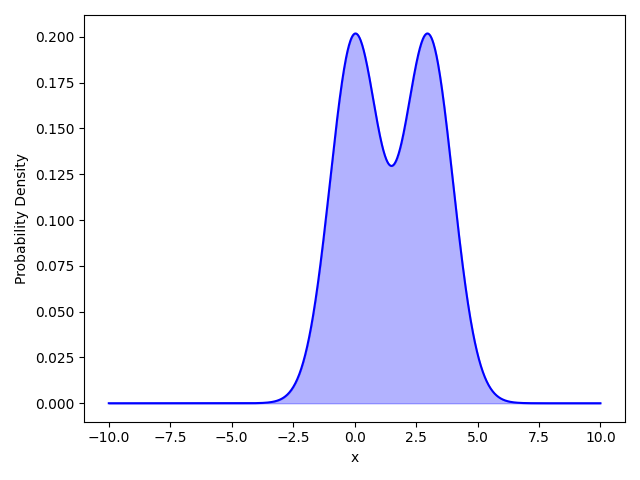
\includegraphics[width=0.5\textwidth]{../images/plot_mixed_normal_distribution.png}
    \caption{Mixed Normal Distribution}
    \label{fig:mixed_normal_distribution}
\end{figure}

\subsubsection{t-Distribution or Student's t-Distribution}\label{t-Distribution or Student's t-Distribution}
The t-distribution, also known as Student's t-distribution, is used in statistical procedures when the sample size is small and the population standard deviation is unknown. It compensates for the underestimation of the standard deviation by the normal distribution in such cases. The t-distribution has wider tails than the normal distribution, which accounts for the increased variability in smaller samples. As the sample size increases, the t-distribution approaches the normal distribution.

The t-distribution is defined as:
\spacedequation{T = \frac{Z}{\sqrt{V/\nu}},}
where $Z$ is a standard normal variable, $V$ is a chi-squared variable with $\nu$ degrees of freedom, and $T$ has an expected value $E=0$ and variance $V=\frac{\nu}{\nu-2}$.

\subsubsection{Cauchy Distribution}\label{Cauchy Distribution}
The Cauchy distribution, also known as the Lorentz distribution, is a continuous probability distribution with heavy tails and undefined mean and variance, often used in physics and spectroscopy. Unlike the normal distribution, the Cauchy distribution does not have a finite mean or variance, which makes it distinct in its applications and properties.

\begin{figure}[h]
    \centering
    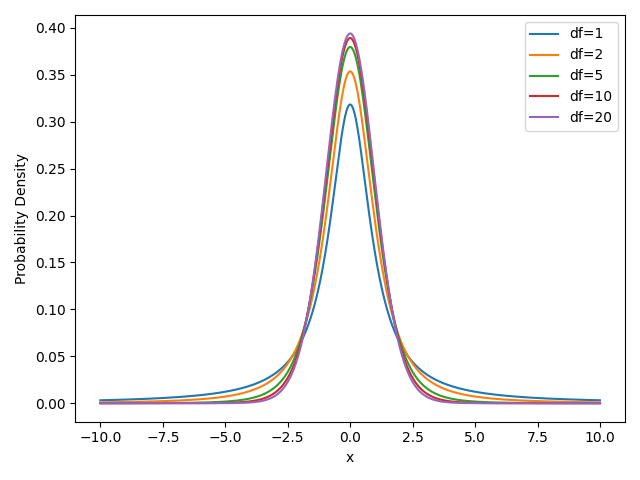
\includegraphics[width=0.5\textwidth]{../images/plot_t_distributions_overlayed.png}
    \caption{t-Distribution}
    \label{fig:t_distribution}
\end{figure}

\subsection{Exponential Distribution}\label{Exponential Distribution}
The exponential distribution is a continuous distribution used to model the duration of random time intervals. The parameter $\lambda$ represents the number of expected \textit{events} per time interval. Examples include the length of a telephone call or radioactive decay. The distribution does not allow negative values, as negative times are meaningless. It is often abbreviated as $\exp(\lambda)$ in statistics. The density function is defined as follows:
\spacedequation{
f_{\lambda}(x) =
\begin{cases}
    \lambda e^{-\lambda x} & \text{if } x \geq 0 \\
    0 & \text{if } x < 0 \\
\end{cases}
}
The expected value $E$ is defined as $\frac{1}{\lambda}$, the variance $V$ as $\frac{1}{\lambda^2}$. The mode (the value at which the probability is highest) of this density function is at $x_{\text{mod}}=0$. If you wish to calculate the probability of the occurrence of an event, it is ideal to use the cumulative distribution function $F(x)$, which forms the integral up to a value $x$. This creates an accumulated probability $P(X\leq x)$. Often, the actual distribution is not an exponential distribution, but the exponential distribution is easy to handle and is applied for simplification. It is applicable when a Poisson process is present, i.e., the Poisson assumptions are fulfilled. The exponential distribution is part of the much larger and more general exponential family, a class of probability measures characterized by ease of handling.

\begin{figure}[h]
    \centering
    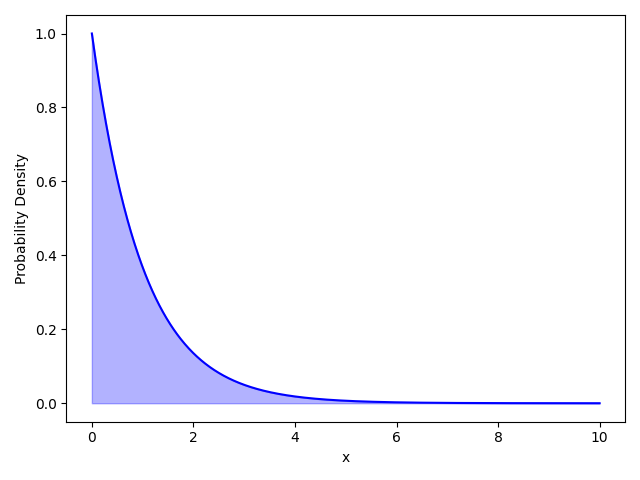
\includegraphics[width=0.5\textwidth]{../images/plot_exponential_distribution.png}
    \caption{Exponential Distribution}
    \label{fig:exponential_distribution}
\end{figure}

\subsubsection{Poisson Distribution}\label{Poisson Distribution}
The Poisson distribution is a discrete probability distribution that describes the distribution of count data. In other words, how often does a certain countable event occur if it is repeated very often? The parameter here indicates the average event rate. The probability for the random variable $X$ of the Poisson distribution is calculated using the following formula:
\spacedequation{P(X=x) = \frac{\lambda^x}{x!} \cdot e^{-\lambda}, \quad x \in \mathbb{N}_0.}
There is a connection between the exponential distribution and the Poisson distribution. Both consider the same phenomenon from different perspectives. The exponential distribution indicates how the probability of the duration of various processes is distributed. The Poisson distribution counts how often the counted events occur in a fixed interval. Starting from the exponential distribution, one wants to determine the probability that exactly $n$ events occur in a time interval of $t$. As will be shown, the result is the Poisson distribution. Since the binomial coefficient for larger values can only be calculated with increased computational effort, one can use the Poisson distribution to approximate the binomial distribution. The Poisson distribution is generally used to approximate the binomial distribution when $n$ is large and $p$ is small. For the expected value $E=\mu$ of the Poisson distribution, we use $\mu=\lambda=n \cdot p$, which is identical to the variance. In general, the Poisson distribution approximates the binomial distribution very well for values of $n \geq 100$ and $\lambda \leq 10$. In addition to the speed advantages in calculation, the Poisson distribution has the advantage that it is countably infinite, thus extending into positive infinity.

\begin{figure}[h]
    \centering
    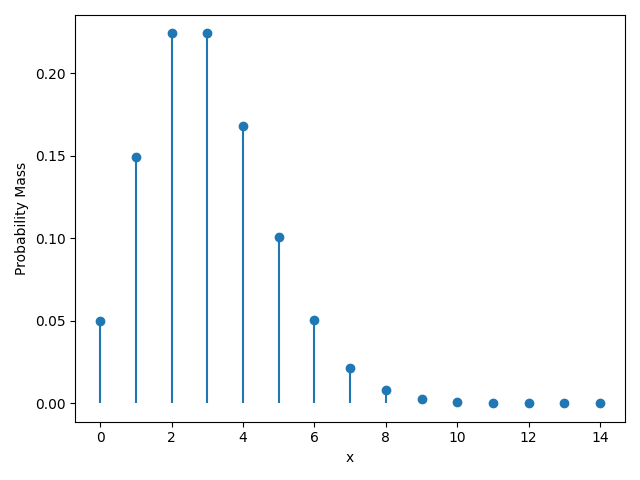
\includegraphics[width=0.5\textwidth]{../images/plot_poisson_distribution.png}
    \caption{Poisson Distribution}
    \label{fig:poisson_distribution}
\end{figure}

\subsubsection{Gamma Distribution}\label{Gamma Distribution}
The gamma distribution is a continuous probability distribution that generalizes the exponential distribution by introducing a shape parameter $\alpha$ and a rate parameter $\beta$. It is often used to model waiting times for multiple events in a Poisson process. The gamma distribution is defined by the following probability density function (PDF):

\spacedequation{
f(x; \alpha, \beta) = \frac{\beta^\alpha x^{\alpha-1} e^{-\beta x}}{\Gamma(\alpha)}, \quad x > 0,
}
where $\Gamma(\alpha)$ is the gamma function, which generalizes the factorial function to non-integer values. The expected value $E$ and variance $V$ of the gamma distribution are given by:

\spacedequation{E = \frac{\alpha}{\beta}, \quad V = \frac{\alpha}{\beta^2}.}

The gamma distribution is particularly useful in Bayesian statistics and reliability engineering, where it is used to model the time until failure of systems with multiple components.

\begin{figure}[h]
    \centering
    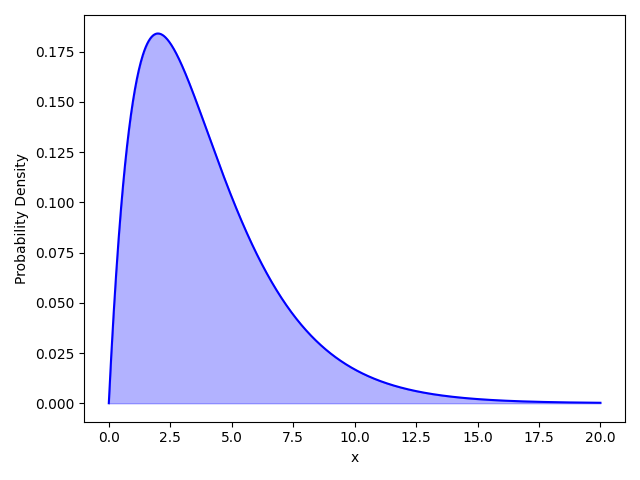
\includegraphics[width=0.5\textwidth]{../images/plot_gamma_distribution.png}
    \caption{Gamma Distribution with $\alpha=2$ and $\beta=1$}
    \label{fig:gamma_distribution}
\end{figure}

\subsubsection{Beta Distribution}\label{Beta Distribution}
The beta distribution is a continuous probability distribution defined on the interval [0, 1], making it suitable for modeling proportions and probabilities. It is characterized by two shape parameters, $\alpha$ and $\beta$, which determine the distribution's shape. The probability density function (PDF) of the beta distribution is given by:

\spacedequation{
f(x; \alpha, \beta) = \frac{x^{\alpha-1} (1-x)^{\beta-1}}{B(\alpha, \beta)}, \quad 0 \leq x \leq 1,
}
where $B(\alpha, \beta)$ is the beta function, which serves as a normalization constant. The expected value $E$ and variance $V$ of the beta distribution are given by:

\spacedequation{E = \frac{\alpha}{\alpha + \beta}, \quad V = \frac{\alpha \beta}{(\alpha + \beta)^2 (\alpha + \beta + 1)}.}

The beta distribution is widely used in Bayesian statistics, particularly as a prior distribution for binomial proportions. It is also used in project management for modeling task completion times and in various fields where probabilities and proportions are analyzed.

\begin{figure}[h]
    \centering
    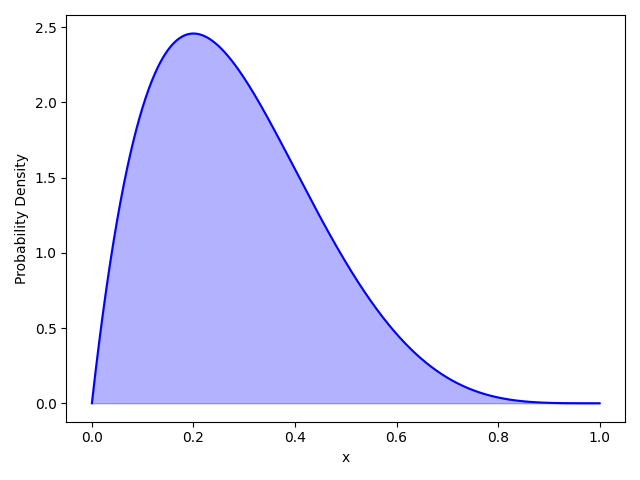
\includegraphics[width=0.5\textwidth]{../images/plot_beta_distribution.png}
    \caption{Beta Distribution with $\alpha=2$ and $\beta=5$}
    \label{fig:beta_distribution}
\end{figure}

\subsubsection{$\chi^2$ Distribution}\label{Chi Square Distribution}
The $\chi^2$ distribution is a continuous distribution often used for testing statistical independence or the validity of a hypothesis (goodness of fit), such as in the \textit{Pearson's chi-square test}~\ref{Pearson's chi-square test}. Very few real-world phenomena are well described by the $\chi^2$ distribution. There is a parameter that defines the degrees of freedom $n$\footnote{If one were to take random independent samples of $n$ normally distributed quantities, these samples would sum to a $\chi^2$ distribution with $n$ degrees of freedom.}. These degrees of freedom determine the distribution insofar as
\spacedequation{\chi_n^2 = Z_1^2 + \dots + Z_n^2}
holds, meaning that $n$ independent, squared, and standard normally distributed random variables are approximately equivalent to it, that is,
\spacedequation{Z_k \sim \mathcal{N}(0,1) \quad \forall k = 1,\dots,n}
and
\spacedequation{\chi^2 \sim \chi_n^2.}
It also holds that
\spacedequation{E_{\chi^2} = n}
and
\spacedequation{V_{\chi^2} = 2 \cdot n.}

\begin{figure}[h]
    \centering
    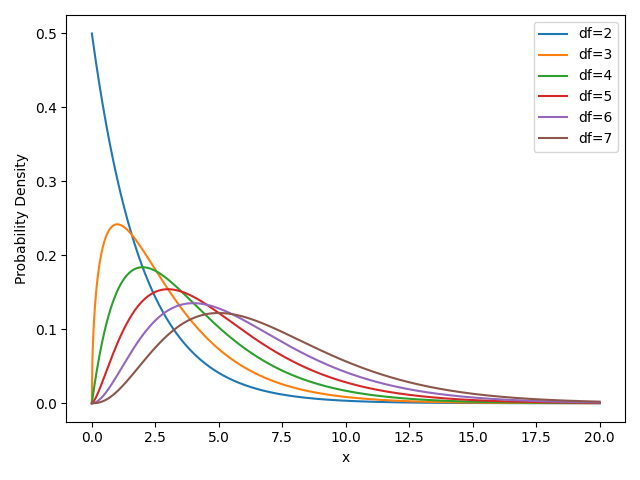
\includegraphics[width=0.5\textwidth]{../images/plot_chi_squared_overlayed.png}
    \caption{$\chi^2$ Distribution}
    \label{fig:chi_square_distribution}
\end{figure}

\subsection{Uniform Distribution}\label{Uniform Distribution}
The French mathematician Pierre Simon de Laplace (1749 to 1827) was one of the first to intensively study random experiments in which it can be assumed that each of its outcomes occurs with the same probability. Random experiments with uniform distribution are called Laplace experiments. The uniform distribution is a special case among probability distributions, as it exists both as a \textit{continuous} and as a \textit{discrete} distribution. Here are briefly the formulas for their calculation. First, for the case of a discrete distribution:
\spacedequation{f(x)=\frac{1}{n}, \quad E(x)=\frac{n+1}{2}, \quad V(x)=\frac{1}{n}\sum_{i=0}^{n}(x_i-\mu)^2.}
And for a continuous distribution:
\spacedequation{
f(x)=
\begin{cases}
    \frac{1}{b-a} & \text{if } a \leq x \leq b \\
    0 & \text{otherwise}. \\
\end{cases}
}
Here, $a$ and $b$ are the boundaries of an interval that includes $x$. Since the same probability applies to all $x$, this depends on the boundaries of the interval
\spacedequation{E(x)=\frac{a+b}{2}, \quad V(x)=\frac{1}{12}(b-a)^2.}

\begin{figure}[h]
    \centering
    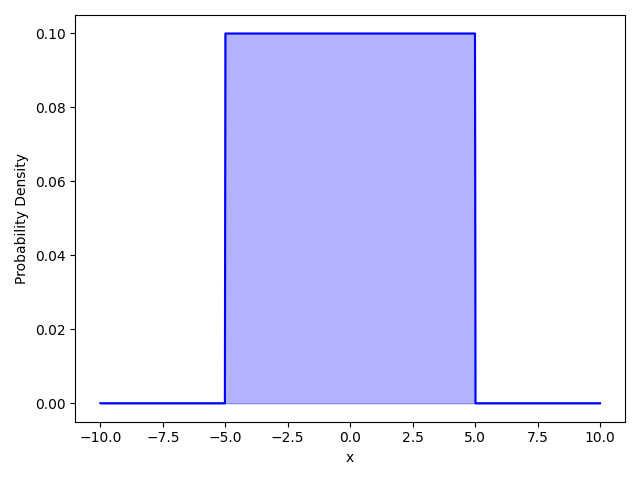
\includegraphics[width=0.5\textwidth]{../images/plot_uniform_distribution.png}
    \caption{Uniform Distribution}
    \label{fig:uniform_distribution}
\end{figure}

\section{Discrete Distributions}\label{Discrete Distributions}
\subsubsection{Binomial Distribution}\label{Binomial Distribution}
Processes in which only two possible outcomes are conceivable (e.g., a coin toss) can be described with the binomial distribution. A prerequisite is that the experiment consists of identical and independent trials. The parameters $n$ and $k$ suggest that this is a discrete probability distribution that answers questions about $k$ successes in $n$ trials. It holds:

\spacedequation{
\begin{tabular}{|c|c|}
    \hline
    Variable & Formula \\
    \hline
    $P(X = k)$ & $\binom{n}{k} p^k (1 - p)^{n - k}$ \\
    $E$ & $n p$ \\
    $V$ & $n p q$ \\
    $\sigma$ & $\sqrt{n p q}$ \\
    $\binom{n}{k}$ & $\dfrac{n!}{k! (n - k)!}$ \\
    \hline
\end{tabular}
}

The binomial coefficient describes the number of ways in which $k$ objects can be arranged in a group of $n$ without repetition. The binomial distribution is left-skewed when $p > 0.5$\footnote{Greater than but not equal to! Symbol missing.}, right-skewed when $p < 0.5$, and symmetric when $p = 0.5$. When $n$ is sufficiently large, the normal distribution can be used as an approximation to the binomial distribution, as the skewness decreases with increasing $n$.

\begin{figure}[h]
    \centering
    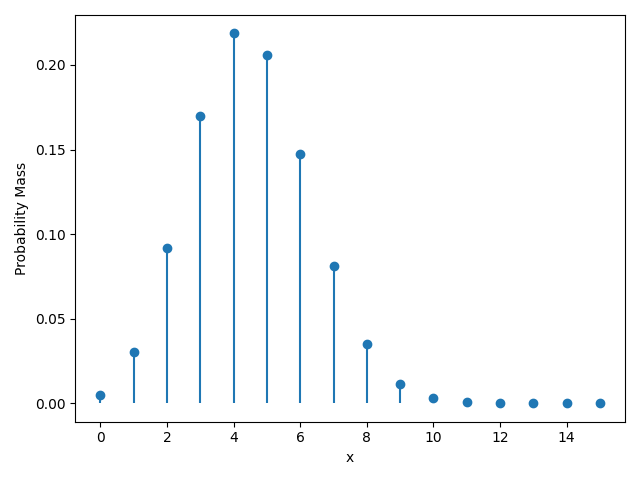
\includegraphics[width=0.5\textwidth]{../images/plot_binomial_distribution.png}
    \caption{Binomial Distribution with $n=15$ and $p=0.3$}
    \label{fig:binomial_distribution}
\end{figure}

\subsubsection{Bernoulli Distribution}\label{Bernoulli}
The Bernoulli distribution is a discrete distribution whose random variable $X$ takes only two values: 0 (failure) or 1 (success). It arises when performing a Bernoulli experiment (which has only two possible outcomes) exactly once. The Bernoulli distribution is therefore a special case of the binomial distribution for $n = 1$.

It holds:
\spacedequation{E_{\text{Bernoulli}} = p,}
\spacedequation{V_{\text{Bernoulli}} = p (1 - p),}
and
\spacedequation{
f_{\text{Bernoulli}}(x) = \begin{cases}
    1 - p & \text{if } x = 0 \\
    p & \text{if } x = 1 \\
    0 & \text{otherwise}. \\
\end{cases}
}

\begin{figure}[h]
    \centering
    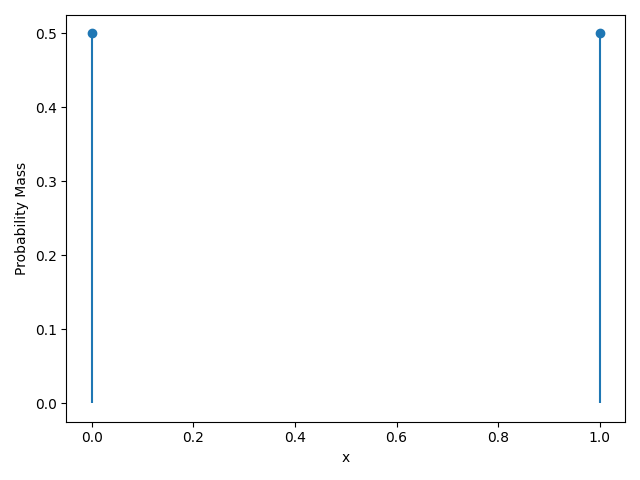
\includegraphics[width=0.5\textwidth]{../images/plot_bernoulli_distribution.png}
    \caption{Bernoulli Distribution with $p=0.5$}
    \label{fig:bernoulli_distribution}
\end{figure}



\section{Maximum Likelihood Estimation}\label{Maximum Likelihood Estimation}
Maximum Likelihood Estimation (MLE) is a method used to estimate the parameters of a statistical model. It works by finding the parameter values that maximize the likelihood function, which measures how well the model explains the observed data. The purpose of MLE is to provide the most likely estimates of the model parameters based on the given data.

The likelihood function $L(\theta)$ for a set of observations $X = \{x_1, x_2, \ldots, x_n\}$ is defined as the joint probability of the observations given the parameters $\theta$:
\spacedequation{L(\theta) = P(X|\theta) = \prod_{i=1}^{n} P(x_i|\theta).}

To find the MLE, we take the natural logarithm of the likelihood function, known as the log-likelihood function $\ell(\theta)$, and then find the parameter values that maximize it:
\spacedequation{\ell(\theta) = \log L(\theta) = \sum_{i=1}^{n} \log P(x_i|\theta).}

The MLE $\hat{\theta}$ is the value of $\theta$ that maximizes $\ell(\theta)$:
\spacedequation{\hat{\theta} = \arg \max_{\theta} \ell(\theta).}

To illustrate MLE, take a look at an animation that shows how the likelihood function changes as the parameter values are adjusted: execute the script found here: \href{../scripts/mle_viz.py}{mle\_viz.py}



\chapter{Statistics}\label{Statistics}

Given data has been collected, one should apply statistical methods to analyze the data and identify assumptions about underlying properties, such as the distribution.
That is the purpose of statistical methods.

\section{Descriptive Statistics}\label{Descriptive Statistics}

\subsubsection{Mean}\label{Mean}
The mean, or average, is the sum of all values in a data set divided by the number of values. It is a measure of central tendency that provides a single value representing the center of the data.
Unlike the expected value $E$ is it used for a finite set of data points, while $E$ is a concept used for random variables and probability distributions. The mean can be seen as a specific case of the expected value when dealing with empirical data.

\subsubsection{Median}\label{Median}
The median is the middle value in a data set when the values are arranged in ascending or descending order. If the data set has an even number of observations, the median is the average of the two middle values.

\subsubsection{Mode}\label{Mode}
The mode is the value that appears most frequently in a data set. It is possible for a data set to have more than one mode if multiple values have the same highest frequency.

\subsubsection{Quantile}\label{Quantile}
Quantiles are cut points that divide the range of a data set into continuous intervals with equal probabilities. Common quantiles include quartiles (dividing data into four parts) and percentiles (dividing data into 100 parts).

\paragraph{Interquartile Range (IQR)}
The interquartile range (IQR) is the range of the middle 50\% of data, calculated as the difference between the third quartile (Q3) and the first quartile (Q1):
\begin{equation}
\text{IQR} = Q_3 - Q_1.
\end{equation}

\subsubsection{Percentile}\label{Percentile}
The percentile indicates the value below which a given percentage of observations in a group of observations falls. For example, the 20th percentile is the value below which 20\% of the observations fall. Percentiles are useful for understanding the relative standing of a value within a data set.

\emptyline
They are calculated by sorting the data set in ascending order and then finding the value below which a certain percentage of the data falls. The formula to find the k-th percentile is:
\begin{equation}
P_k = \left( \frac{k}{100} \right) (n + 1),
\end{equation}
where $P_k$ is the k-th percentile, $k$ is the desired percentile, and $n$ is the number of observations in the data set.

\subsection{Categorical Variables}\label{Categorical Variables}
\subsubsection{Nominal}\label{Nominal}
Nominal data represents categories without any intrinsic ordering. Examples include gender, race, and the presence or absence of a feature.

\subsubsection{Ordinal}\label{Ordinal}
Ordinal data represents categories with a meaningful order but no consistent difference between categories. Examples include rankings, such as class grades (A, B, C, etc.) or levels of satisfaction (satisfied, neutral, dissatisfied).

\section{Hypothesis Testing}\label{Hypothesis Testing}

\subsection{Concepts and Terminology}\label{Concepts and Terminology}

Hypothesis testing is a statistical method used to make decisions about the properties of a population based on a sample of data. It involves formulating two competing hypotheses: the null hypothesis (\(H_0\)) and the alternative hypothesis (\(H_1\) or \(H_a\)). The null hypothesis represents a statement of no effect or no difference, while the alternative hypothesis represents a statement of an effect or difference.
\begin{enumerate}
    \item [1.] Formulate the null and alternative hypotheses.
    \item [2.] Choose a significance level (\(\alpha\)), which is the probability of rejecting the null hypothesis when it is true.
    \item [3.] Collect and summarize the sample data into a test statistic.
    \item [4.] Determine the p-value, which is the probability of obtaining a test statistic at least as extreme as the one observed, assuming the null hypothesis is true.
    \item [5.] Compare the p-value to the significance level to decide whether to reject or fail to reject the null hypothesis.
\end{enumerate}
    
If the p-value is less than or equal to the significance level, the null hypothesis is rejected in favor of the alternative hypothesis. Otherwise, there is not enough evidence to reject the null hypothesis.

\subsubsection{p-value}
The p-value is the probability of obtaining a test statistic at least as extreme as the one observed, assuming the null hypothesis is true. If the p-value is less than or equal to the significance level (\(\alpha\)), the null hypothesis is rejected.

\subsubsection{Significance Level (\(\alpha\))}
The significance level (\(\alpha\)) is the probability of rejecting the null hypothesis when it is true. Common choices for \(\alpha\) are 0.05, 0.01, and 0.10.

\subsubsection{Type I and Type II Errors}
A Type I error occurs when the null hypothesis is rejected when it is true (false positive). A Type II error occurs when the null hypothesis is not rejected when it is false (false negative).

\begin{figure}[h]
    \centering
    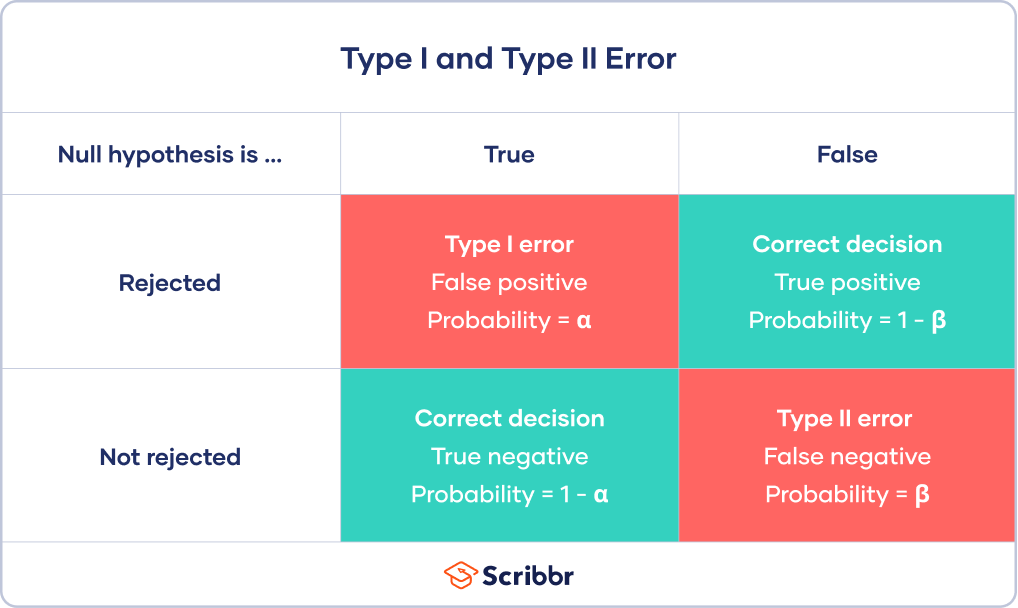
\includegraphics[width=0.6\textwidth]{../images/type-i-and-ii-error-2.png}
    \caption{Type I and Type II Errors
    {\url{https://www.scribbr.com/statistics/type-i-and-type-ii-errors/}}.}
    \label{fig:Type I and Type II Errors}
\end{figure}

\section{Test Statistic}
The test statistic is calculated from the sample data and is used to determine whether to reject the null hypothesis. The type of test statistic depends on the test being used (e.g., z-test, t-test).

\subsection{z-test}
The z-test is used for large sample sizes or when the population variance is known. It tests whether the sample mean is significantly different from the population mean.
\spacedequation{z = \frac{\bar{X} - \mu}{\sigma / \sqrt{n}},}
where $\bar{X}$ is the sample mean, $\mu$ is the population mean, $\sigma$ is the population standard deviation, and $n$ is the sample size.

\subsection{t-test}
The t-test is used for small sample sizes or when the population variance is unknown. There are different types of t-tests, including one-sample, two-sample, and paired t-tests.

\subsubsection{One-Sample t-test}
The one-sample t-test is used to determine whether the mean of a single sample is significantly different from a known or hypothesized population mean.
\spacedequation{t = \frac{\bar{X} - \mu}{s / \sqrt{n}},}
where $\bar{X}$ is the sample mean, $\mu$ is the population mean, $s$ is the sample standard deviation, and $n$ is the sample size.

\subsubsection{Two-Sample t-test}
The two-sample t-test (independent t-test) is used to compare the means of two independent samples to determine if they are significantly different from each other.
\spacedequation{t = \frac{\bar{X}_1 - \bar{X}_2}{\sqrt{\frac{s_1^2}{n_1} + \frac{s_2^2}{n_2}}},}
where $\bar{X}_1$ and $\bar{X}_2$ are the sample means, $s_1$ and $s_2$ are the sample standard deviations, and $n_1$ and $n_2$ are the sample sizes of the two groups.

\subsubsection{Paired t-test}
The paired t-test is used to compare the means of two related groups. It is often used in before-and-after studies or when the samples are matched pairs.
\spacedequation{t = \frac{\bar{D}}{s_D / \sqrt{n}},}
where $\bar{D}$ is the mean of the differences between paired observations, $s_D$ is the standard deviation of the differences, and $n$ is the number of pairs.

\subsection{Chi-square test}
\subsubsection{Chi-Square Test for Independence}
The Chi-Square Test for Independence tests if there is an association between two categorical variables. It compares the observed frequencies in each category of a contingency table to the frequencies expected if the variables were independent.
\spacedequation{\chi^2 = \sum \frac{(O_{ij} - E_{ij})^2}{E_{ij}},}
where $O_{ij}$ is the observed frequency in the $i$-th row and $j$-th column, and $E_{ij}$ is the expected frequency in the $i$-th row and $j$-th column.

\subsubsection{Chi-Square Goodness of Fit}
The Chi-Square Goodness of Fit test determines if observed frequencies match expected frequencies for a single categorical variable. It assesses how well the observed distribution of data fits with the distribution expected under a specific hypothesis.
\spacedequation{\chi^2 = \sum \frac{(O_i - E_i)^2}{E_i},}
where $O_i$ is the observed frequency and $E_i$ is the expected frequency for the $i$-th category.

\subsection{ANOVA (Analysis of Variance)}
ANOVA is used to compare means among three or more groups to see if at least one group mean is different from the others. It analyzes the variance within groups and between groups.

\subsubsection{One-Way ANOVA}
One-way ANOVA is used when there is one independent variable with multiple levels (groups). It tests whether there are any statistically significant differences between the means of three or more independent (unrelated) groups.
\spacedequation{F = \frac{\text{variance between groups}}{\text{variance within groups}}.}

\subsubsection{Two-Way ANOVA}
Two-way ANOVA is used when there are two independent variables. It tests the effect of two factors simultaneously and also examines the interaction between the two factors.
\spacedequation{F = \frac{\text{variance due to factor A, factor B, and interaction}}{\text{variance within groups}}.}

\subsection{F-Test}
The F-test is used to compare the variances of two groups to determine if they are significantly different. It is based on the ratio of the two sample variances.
\begin{equation}
F = \frac{s_1^2}{s_2^2},
\end{equation}
where $s_1^2$ and $s_2^2$ are the sample variances of the two groups.

\subsection{Levene’s Test}
Levene’s Test is used to check for equality of variances across groups. It is more robust to departures from normality than the F-test. The test statistic is calculated as:
\begin{equation}
W = \frac{(N - k)}{(k - 1)} \frac{\sum_{i=1}^k N_i (Z_{i\cdot} - Z_{\cdot\cdot})^2}{\sum_{i=1}^k \sum_{j=1}^{N_i} (Z_{ij} - Z_{i\cdot})^2},
\end{equation}
where $Z_{ij} = |Y_{ij} - \bar{Y}_i|$, $Y_{ij}$ is the value of the $j$-th case in the $i$-th group, $\bar{Y}_i$ is the mean of the $i$-th group, $Z_{i\cdot}$ is the mean of the $Z_{ij}$ in the $i$-th group, and $Z_{\cdot\cdot}$ is the mean of all $Z_{ij}$.


\subsection{Pearson Correlation Coefficient}\label{Pearson Correlation Coefficient}
In statistical analysis, the relationship between the independent and dependent variables can be analyzed using various methods such as correlation and regression analysis. The correlation coefficient $r$ measures the strength and direction of the linear relationship between two variables:
\spacedequation{r = \frac{\sum (X_i - \bar{X})(Y_i - \bar{Y})}{\sqrt{\sum (X_i - \bar{X})^2 \sum (Y_i - \bar{Y})^2}},}
where $X_i$ and $Y_i$ are the individual sample points, and $\bar{X}$ and $\bar{Y}$ are the means of $X$ and $Y$ respectively.

\emptyline
These are basic statistical methods not needing much computational power. However, a layer deeper statisticians build models to describe their observations.  
Because it is beyond the scope of this chapter, it will not discuss it here.
\input{Geometry.tex}
\input{Linear Algebra.tex}
\input{Analysis.tex}
\input{Machine Learning.tex}

\end{document}
